%Update 2020: Meritxell
\documentclass[11pt,a4paper]{article}
% Packages
\usepackage[latin1]{inputenc}
%\usepackage[english]{babel}
\usepackage{graphicx}
\usepackage{amsmath}
\usepackage{hyperref}
\usepackage{verbatim}
\usepackage{listings}
\usepackage{xcolor}
\usepackage{float}
\usepackage{chngcntr}
\usepackage[framed,numbered,autolinebreaks,useliterate]{mcode}
\usepackage{url}
\usepackage{afterpage}


%Subsection of the form 1.a instead of 1.1
\counterwithin*{subsection}{section}
\renewcommand{\thesubsection}{\thesection.\alph{subsection}}

%Add a blank page
\newcommand\blankpage{%
    \null
    \newpage}


\definecolor{codegreen}{rgb}{0,0.6,0}
\definecolor{codegray}{rgb}{0.5,0.5,0.5}
\definecolor{codepurple}{rgb}{0.58,0,0.82}
\definecolor{backcolour}{rgb}{0.95,0.95,0.92}

\lstdefinestyle{mystyle}{
    backgroundcolor=\color{backcolour},   
    commentstyle=\color{codegreen},
    keywordstyle=\color{magenta},
    numberstyle=\tiny\color{codegray},
    %identifierstyle=\color{blue},
    stringstyle=\color{codepurple},
    basicstyle=\ttfamily\footnotesize,
    breakatwhitespace=false,         
    breaklines=true,                 
    captionpos=b,                    
    keepspaces=true,                 
    numbers=left,                    
    numbersep=5pt,                  
    showspaces=false,                
    showstringspaces=false,
    showtabs=false,                  
    tabsize=2
}

\lstset{style=mystyle}

%% Format de la page
\pagestyle{plain}
%\setlength{\hoffset}{-0.4mm}
%\setlength{\voffset}{-1.4mm}%{-5.4mm}
\setlength{\oddsidemargin}{0mm}
%\setlength{\topmargin}{0mm}
%\setlength{\headheight}{0mm}
%\setlength{\headsep}{0mm}
\setlength{\textheight}{225mm}
\setlength{\textwidth}{160mm}
\newlength{\thickness} \setlength{\thickness}{0.2mm}
\setlength{\parindent}{0cm}
%\setlength{\parskip}{4pt}

\title{Project_1}
\author{raphael.mirallie }
\date{December 2020}

\begin{document}
\noindent \parbox[b]{12 cm}{
  \small
{\bf EPFL, Swiss Federal Institute of Technology in Lausanne} \\
{\bf SMA}

\bigskip

{\bf Numerical methods for conservation Laws}\\
{\bf Dr. Deep Ray}\\
{\bf Fall 2020}

} \hfill 
\includegraphics[width=4cm]{epfl_logo.jpg}

\noindent\hrulefill\\
\centerline{\large \bf One-dimensional shallow water equation using finite volume method}\vspace{2ex}
\centerline{\bf Project 1}
\centerline{\bf  Axel Dinh Van Chi, Rapha\"el Miralli\'e}


%--------------------------------------------------------------------
\graphicspath{ {pictures/} }

\section{Question 1}
\subsection{}

An uniform discretization of $\Omega$ was used. Let's define $\mathbf{q}=\begin{pmatrix} h \\ m \end{pmatrix}$ and $u=\frac{m}{h}$. The Lax-Friedrichs (LF) flux is given by:

\[F_{j+\frac{1}{2}}(\mathbf{q}_l,\mathbf{q}_r)=\frac{f(\mathbf{q}_l)+f(\mathbf{q}_r)}{2} - |\lambda_{max}|\frac{\mathbf{q}_l+\mathbf{q}_r}{2}\] 

where $\lambda_{max}=max\{|u_l|+\sqrt{h_l},|u_r|+\sqrt{h_r}\}$ are the eigenvalue of $f$.
The code used can be found in \ref{plot_sol} with Initial\_conditions set to 1.

\subsection{}
The numerical solution of the LF method at $T=2$ is shown in Figure \ref{fig:IC_1_100_cells} (100 cells mesh) and in Figure \ref{fig:IC_1_1000_cells} (1000 cells mesh). Corresponding code can be found in \ref{plot_err}.

The norm used to calculate the error is the $\| . \|_{h,2}$ (where $h=\frac{2}{N}$) norm as defined in the lecture, i.e :
\[ \|u\|_{h,p} = (h\sum_j |u_j|^p)^{\frac{1}{p}}\]
with $p=2$. The same norm will be used for all of the projects, but the code has be adapted to be able to choose any $p \in (1,\infty).$

The error is expressed in Figure \ref{fig:IC_1_errors} with respect to the number of cells $N$ (note that $\Delta x = \frac{1}{N}$). The error is calculated with a reference solution set with a mesh of 10 000 cells. The solution converges in $O(h)$, as expected. 



%--------------------------------------------------------------------

\section{Question 2}
\subsection{}
The plot for IC (5) and (6) are Figure \ref{fig:IC_2_100_cells} and \ref{fig:IC_3_250_cells} respectively. With initial conditions (IC) (5), the scheme produce a smooth solution that converges in $O(h)$ as expected. However, with IC (6), the scheme leads to discontinuous solution, with periodic discontinuity points. In particular, the LF scheme is not able to get sharp discontinuities and smoothen them (e.g. at $x \approx 1.5$) . As for IC (5), the LF scheme does way better in smooth areas. This issue will be dealt with with the implementation of the Roe linearization in the Godunov scheme.


\subsection{}
The plot of the error is shown in Figure \ref{fig:IC_2_errors} and in Figure \ref{fig:IC_3_errors} for IC (5) and (6) respectively.


%--------------------------------------------------------------------

\section{Question 3}
\subsection{}
Godunov needs rieman pb solution, to do so we need a linear problem, thus Roe linearization 
\subsection{}
We consider the one-dimensional shallow water equation as follow :
\[ \bf{q}_t+\bf{f}_x=0\]
and we are looking for $\hat{A}$ such that :
\[\hat{A}(\bf{q}_r-q_l)=(f_r-f_l)\]
Let's introduce $\mathbf{z}=h^{-1/2}\mathbf{q}$ such that we can express the jump in \textbf{q} and \textbf{f} can be expressed in terms of the jump in \textbf{z}. We are gonna use the following identity : $\Delta(ab)=\overline{a}\Delta(b)+\overline{b}\Delta(a)$. We then have:


\begin{equation*}
     \mathbf{q} = \begin{pmatrix} h \\ m \end{pmatrix} = \begin{pmatrix} z_1^2 \\ z_1z_2 \end{pmatrix}, \quad
     \Delta \mathbf{q} = \begin{pmatrix} \Delta z_1^2 \\  \Delta z_1z_2 \end{pmatrix} = \begin{pmatrix} 2\overline{z_1}\Delta z_1 \\   \overline{z_1}\Delta z_2+\overline{z_2}\Delta z_1 \end{pmatrix} ,\quad
     f(\mathbf{z})= \begin{pmatrix} z_1z_2 \\   z_1+\frac{g}{2}z_1^4 \end{pmatrix}
\end{equation*}
\begin{equation*}
    \Delta f(\mathbf{z})= \begin{pmatrix} \overline{z_1}\Delta z_2+\overline{z_2}\Delta z_1 \\   2\overline{z_2}\Delta z_2 + 2g\overline{z_1}\overline{z_1^2}\Delta z_1 \end{pmatrix},
\end{equation*}
\\
We now want to find $B$ and $C$ such that $\Delta \mathbf{q}=B\Delta \mathbf{z}$ and $\Delta f(\mathbf{z})=C\Delta\mathbf{z}$. Using the previous relations we find:

\begin{equation}
    B = \begin{pmatrix} 2\overline{z_1} & 0 \\ \overline{z_2} & \overline{z_2}\end{pmatrix} \ \text{and} \ C = \begin{pmatrix} \overline{z_2} & \overline{z_1} \\ 2g\overline{z_1}\overline{z_1^2} & 2\overline{z_2}\end{pmatrix}
\end{equation}
And that leads us to: 
\begin{equation}
    \hat{A}=CB^{-1} = \begin{pmatrix} 0 & 1 \\ g\overline{z_1^2}-(\overline{z_2^2})(\overline{z_1^1})^{-2} & 2(\overline{z_2})(\overline{z_1})^{-1}\end{pmatrix} 
\end{equation}

\subsection{}

The Godunov flux with Roe linearization is given by 
\[F_{j+\frac{1}{2}}(\mathbf{q}_l,\mathbf{q}_r)=\frac{f(\mathbf{q}_l)+f(\mathbf{q}_r)}{2} - |A^*|\frac{\mathbf{q}_l+\mathbf{q}_r}{2}\] where $|A^*|$ is the Roe linearization. In our case $A^*=\hat{A}$. Thus we need to diagonalize $\hat{A}$ to compute $|A^*|$. From the diagolanization we find $\Lambda$ the diagonal matrix of eigenvalue of $A^*$ and $S$ the matrix of the corresponding eigenvector. We now have $|A^*|=S|\Lambda|S^{-1}$. The corresponding code can be found in \ref{G_flux} and \ref{rhs}.

\subsection{}

See Figure \ref{fig:IC_1_100_cells}, \ref{fig:IC_2_100_cells} and \ref{fig:IC_3_250_cells} for the solution at T=2 with initial conditions (2), (5) and (6) respectively. 
\ref{fig:IC_1_errors},\ref{fig:IC_2_errors} and \ref{fig:IC_3_errors} for the error of the scheme compare to a mesh of 10 000 cells with initial conditions (2), (5) and (6) respectively.

\subsection{}
In this subsection, we will consider that not violation of the entropy condition appears. The accuracy of the LF and Roe scheme is almost identical for smooth solutions. However, when the solution has discontinuities, the Roe scheme is able to approximate these discontinuities in a much better way than the LF scheme. Thus the accuracy of the Roe scheme is better when facing punctual discontinuity, but is equivalent for smooth solutions. 

%------------------------------------------------------------------------

\section{Question 4}

\subsection{}
The reference solutions was obtained with a mesh of 10 000 cells. 

\subsection{}
Plots can be found in Figure \ref{fig:IC_4_100_cells} and Figure \ref{fig:IC_4_1000_cells}. 
\subsection{}
The Roe solution can be found in the same Figure as above. We can clearly see that the Roe solution is not the same as before. It doesn't converge to the LF scheme reference. Indeed 

%------------------------------------------------------------------------
\newpage
\section{Figures}
%IC 1
\begin{figure}[!htb]
    \centering
    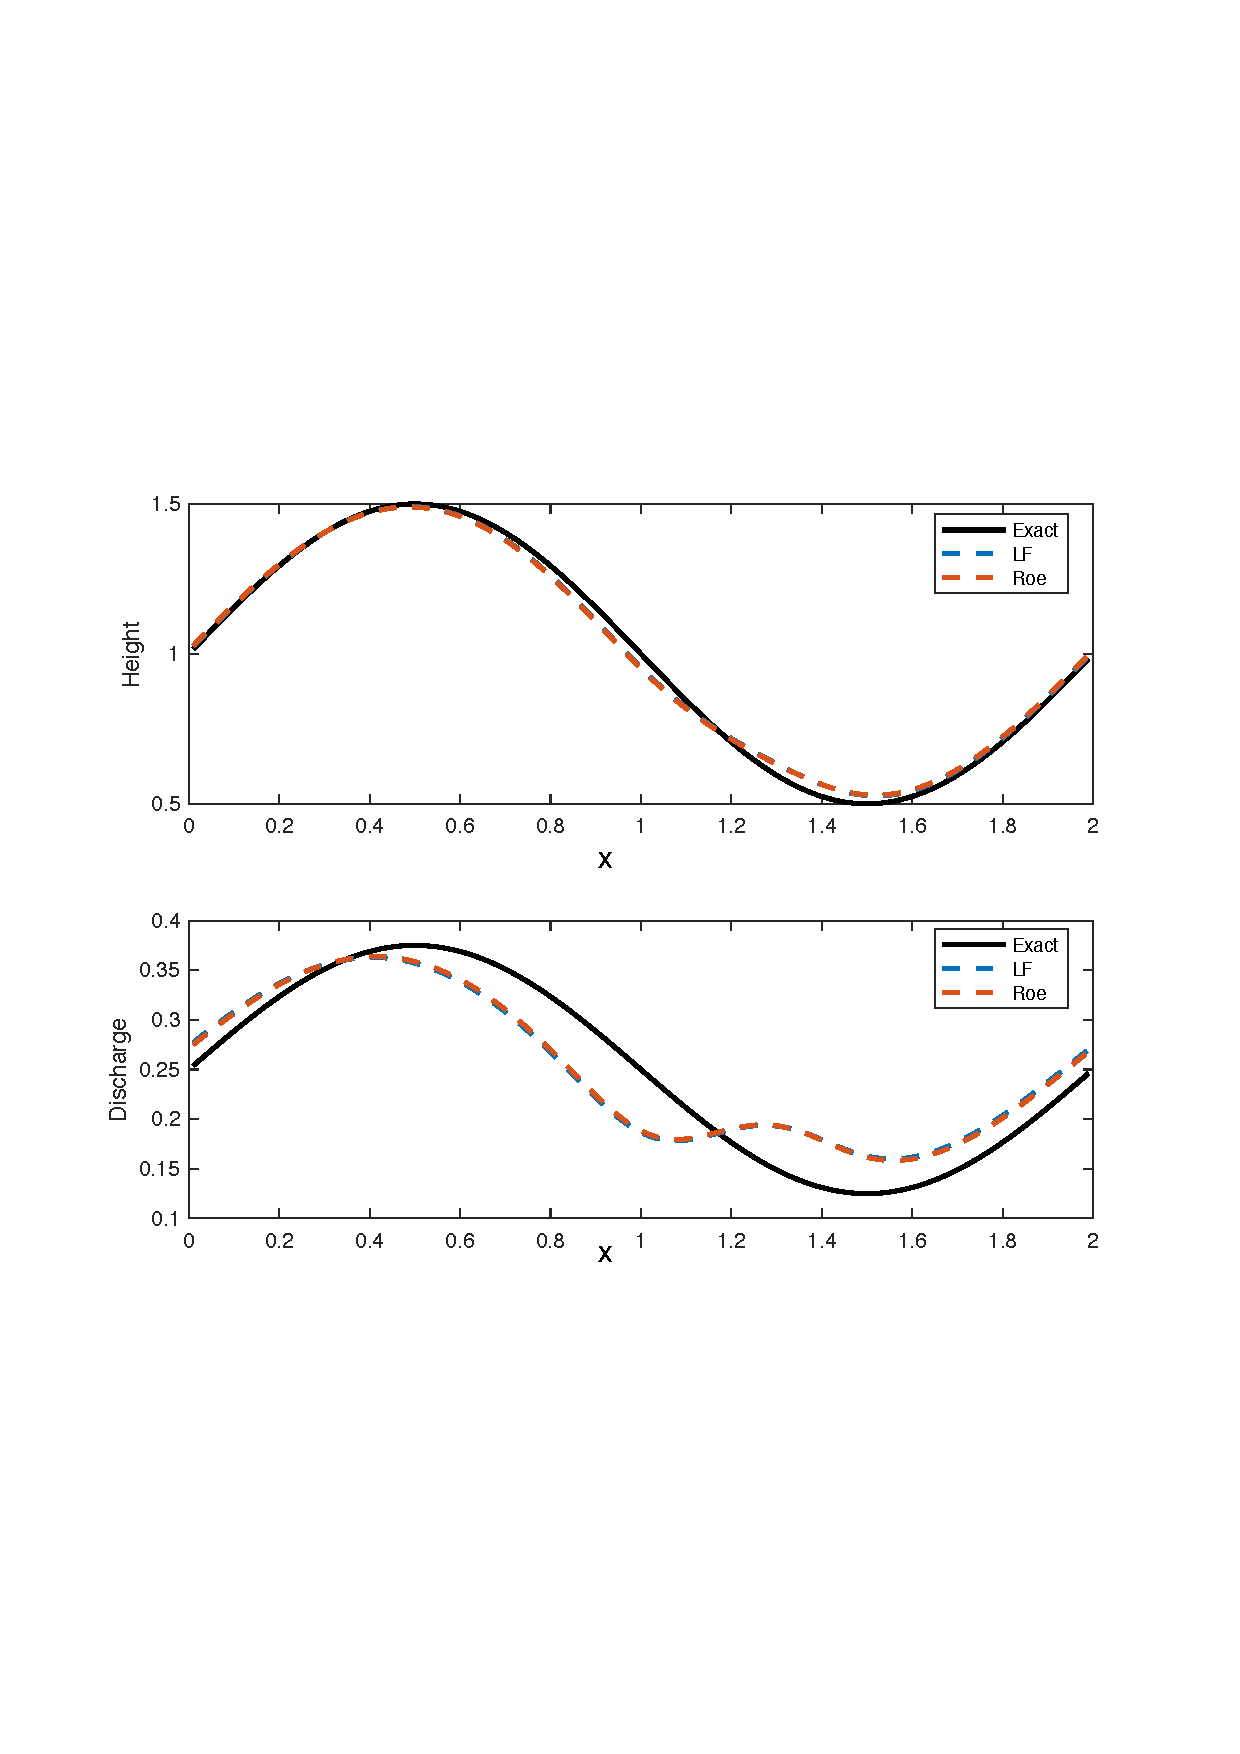
\includegraphics[width=11cm]{pictures/IC_1_100_cells.pdf}
    \caption{LF and Roe methods, 100 cells, IC (2)}
    \label{fig:IC_1_100_cells}
\end{figure}

\begin{figure}[!htb]
    \centering
    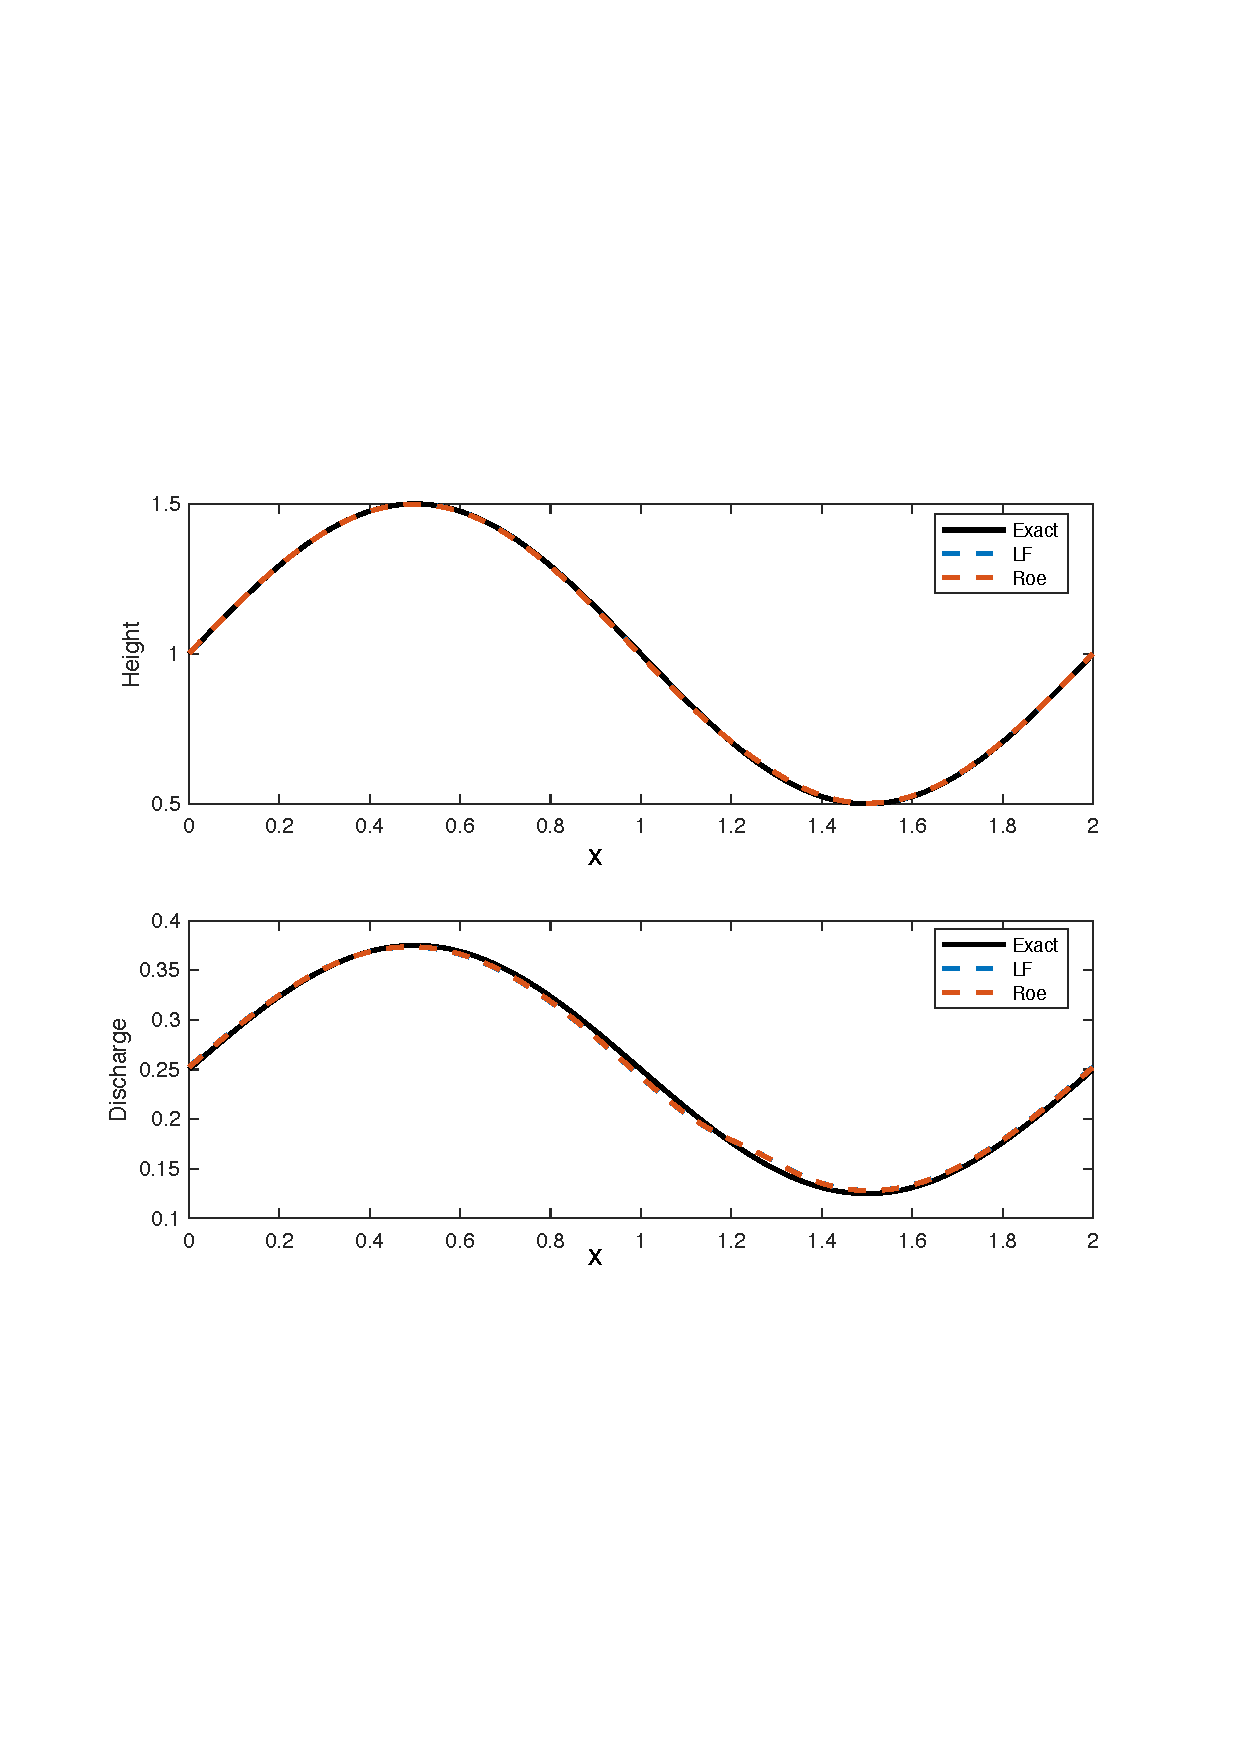
\includegraphics[width=11cm]{pictures/IC_1_1000_cells.pdf}
    \caption{LF and Roe methods, 1000 cells, IC (2)}
    \label{fig:IC_1_1000_cells}
\end{figure}

\begin{figure}[!htb]
    \centering
    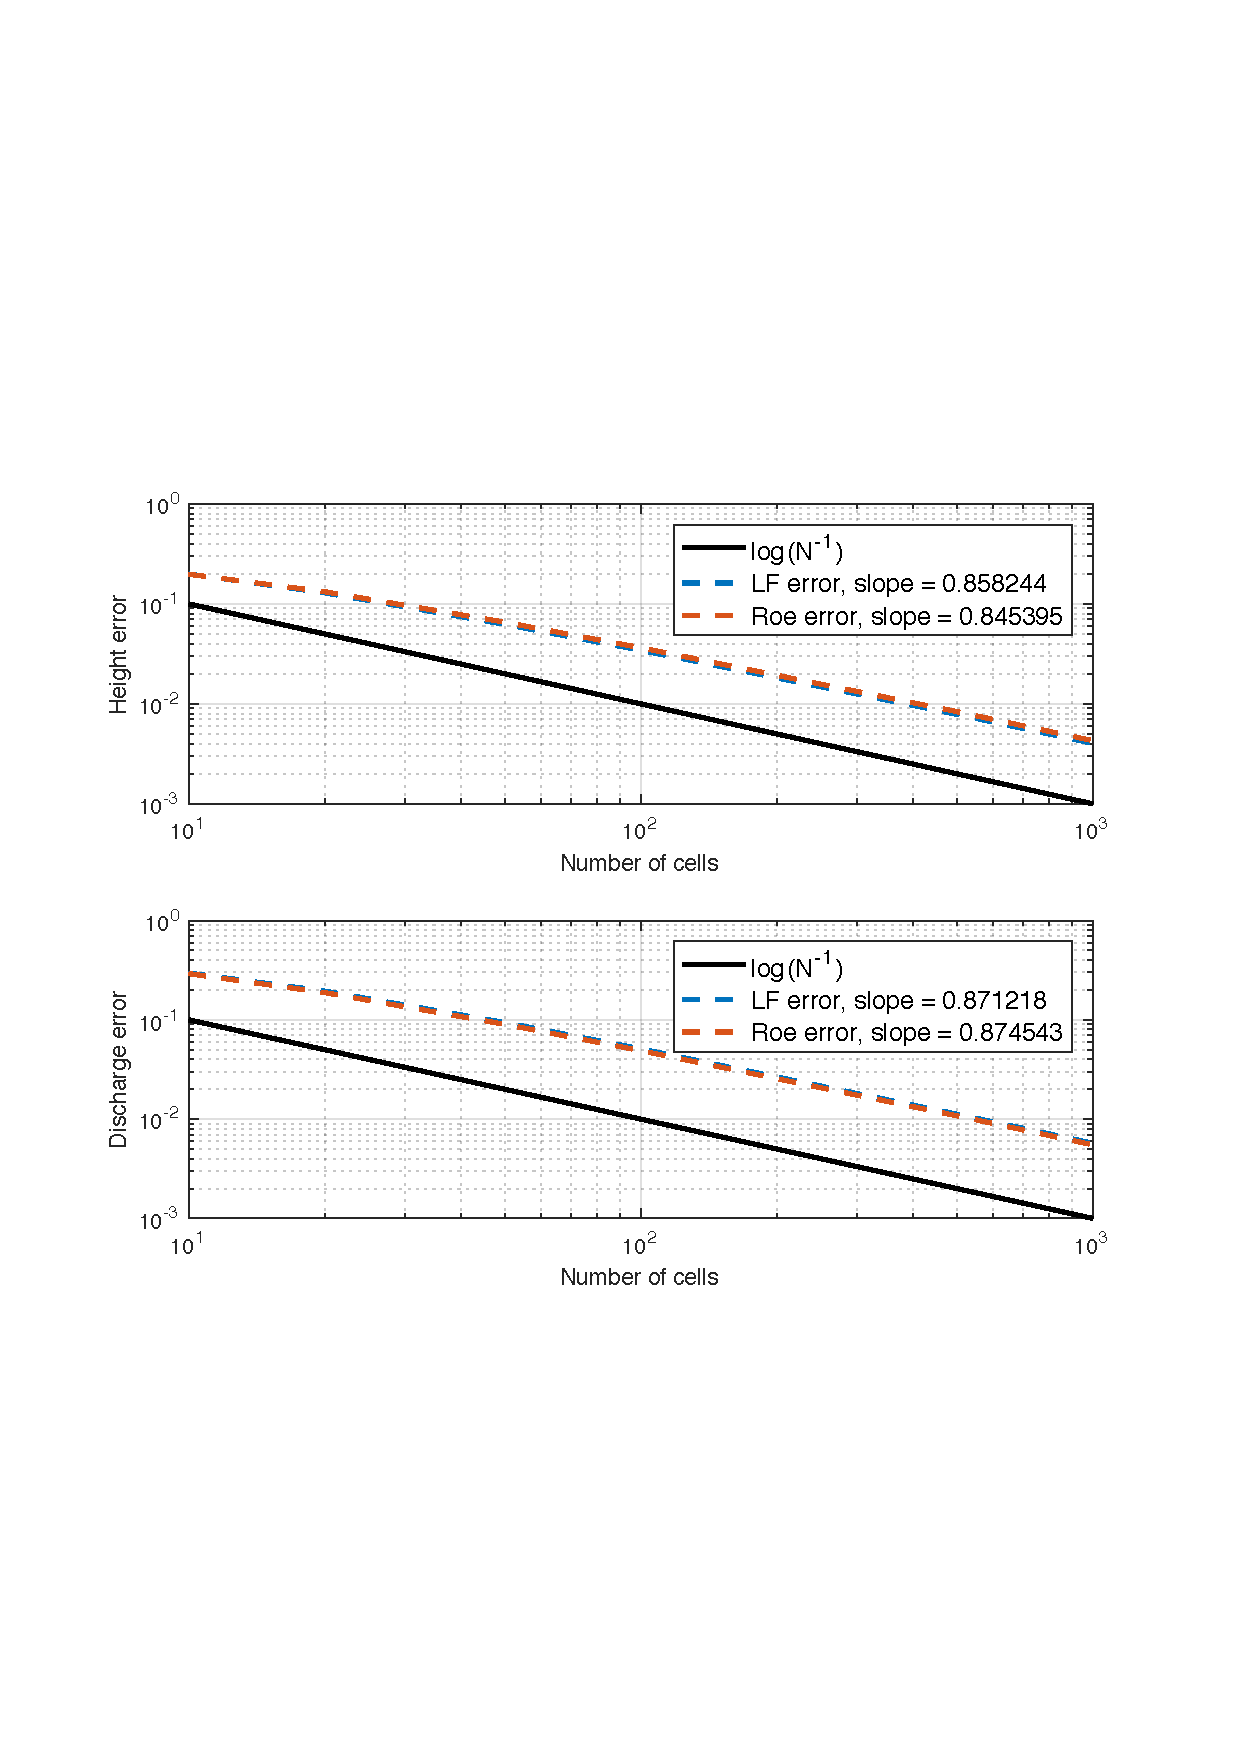
\includegraphics[width=11cm]{pictures/IC_1_error.pdf}
    \caption{LF and Roe methods errors, IC (2)}
    \label{fig:IC_1_errors}
\end{figure}

%IC 2
\begin{figure}[!htb]
    \centering
    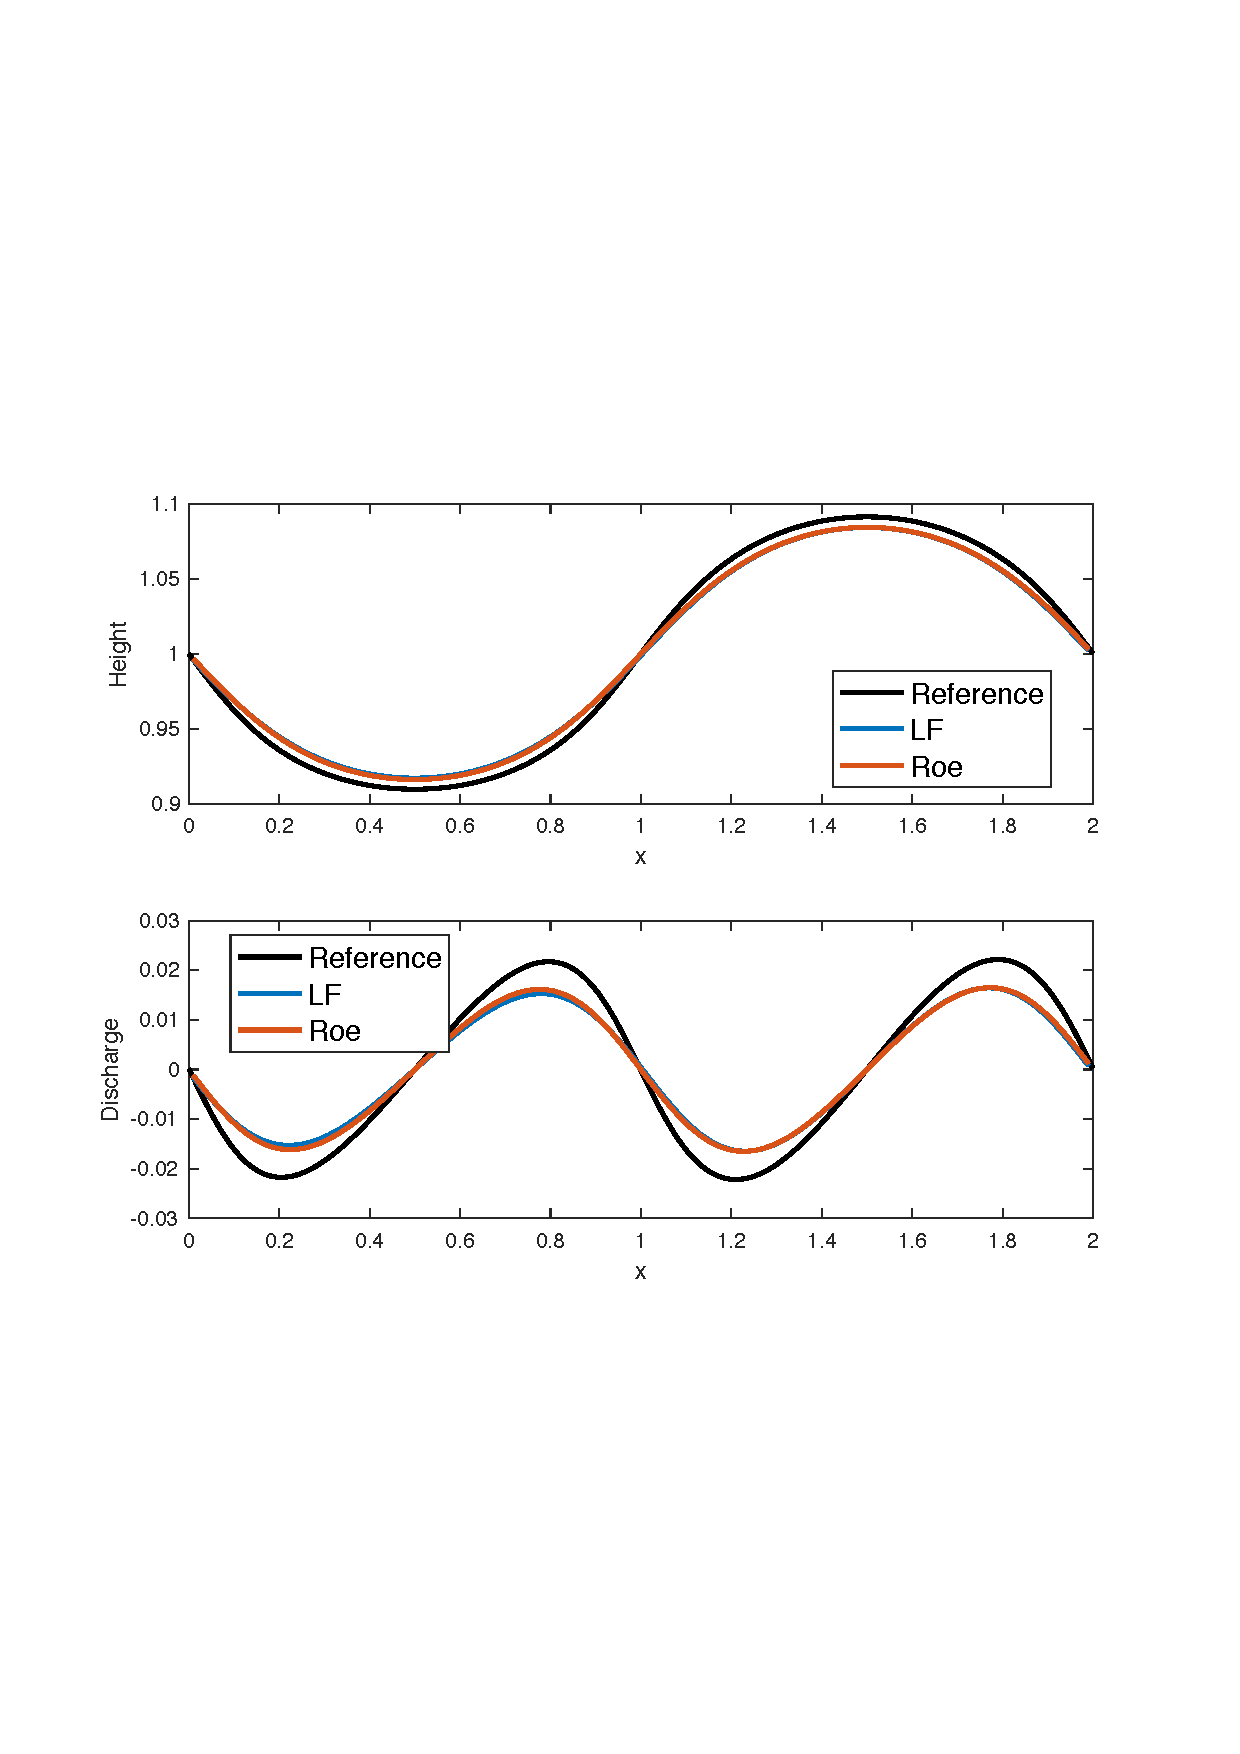
\includegraphics[width=11cm]{pictures/IC_2_100_cells.pdf}
    \caption{LF and Roe methods, 100 cells, IC (5)}
    \label{fig:IC_2_100_cells}
\end{figure}

\begin{figure}[!htb]
    \centering
    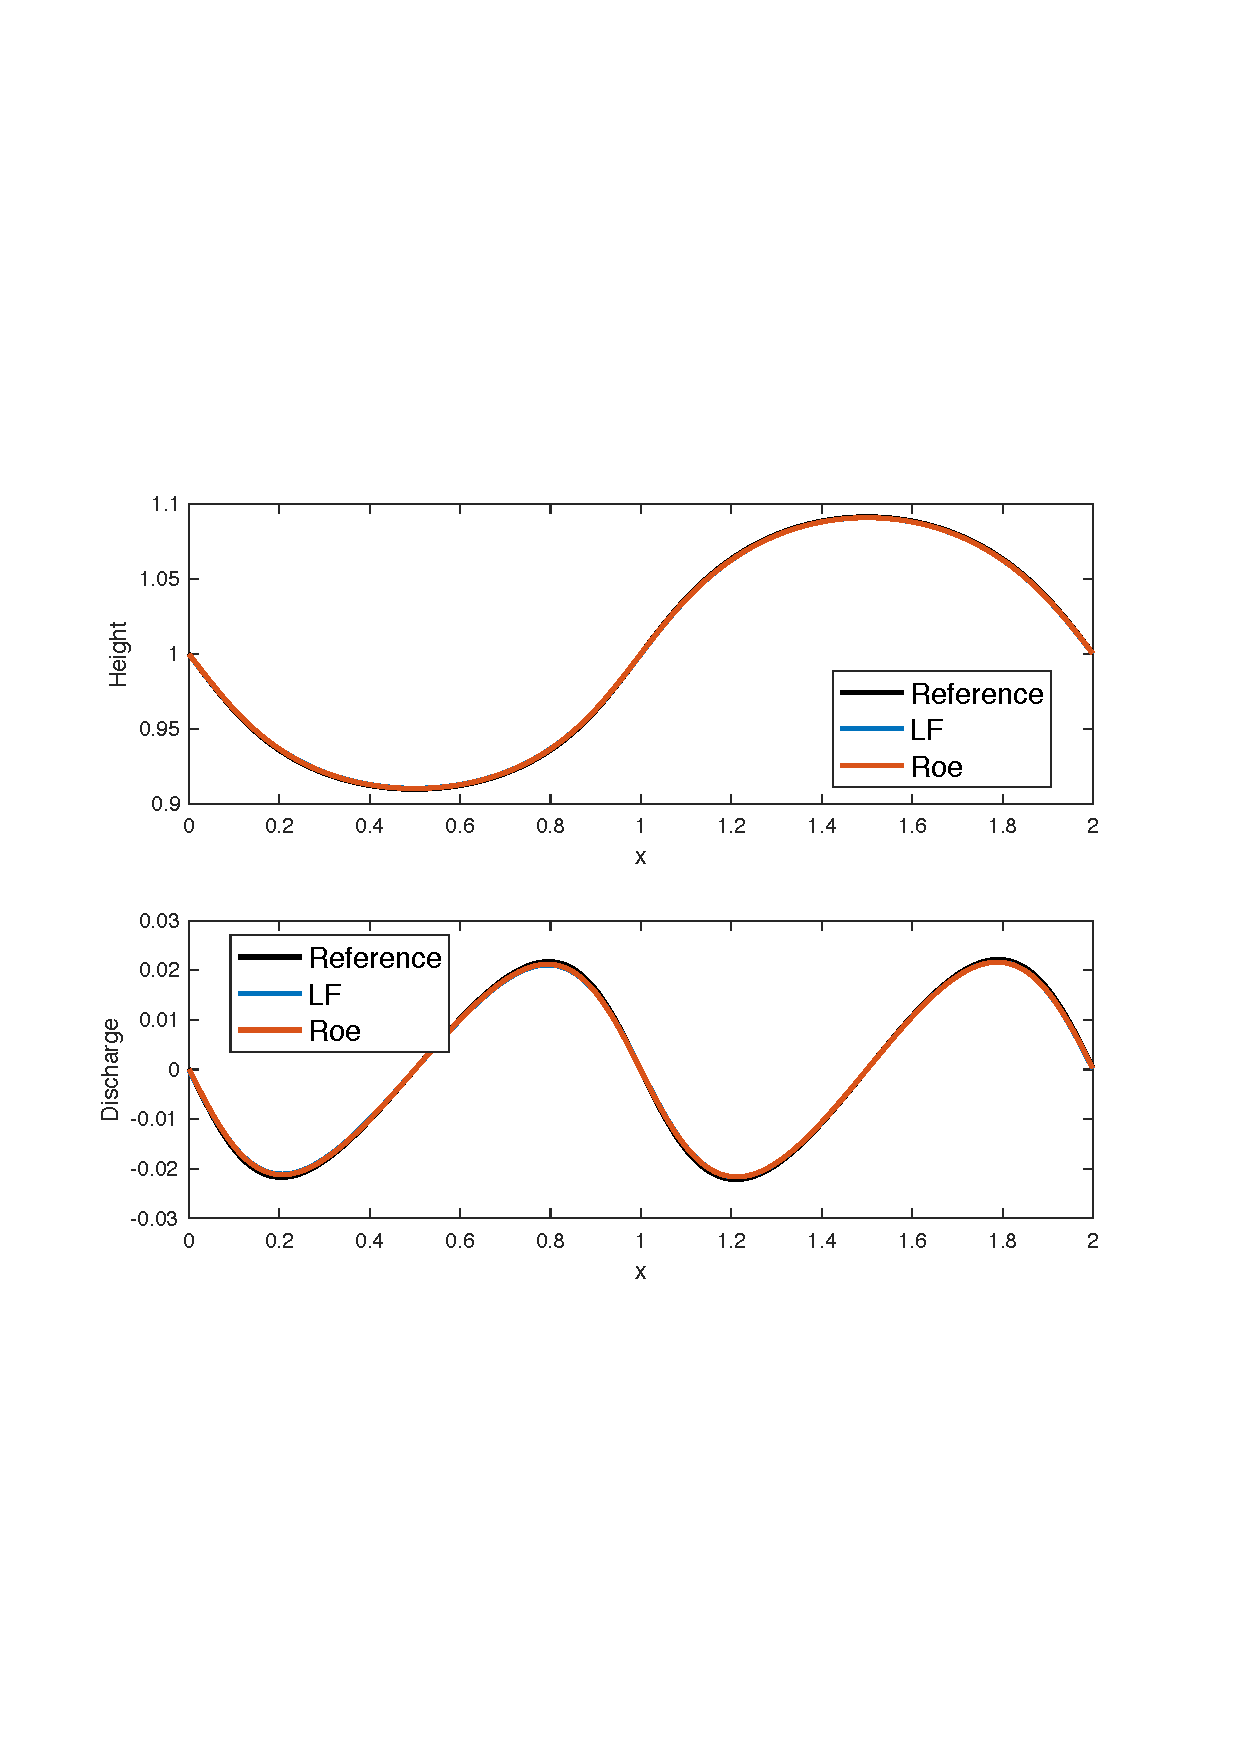
\includegraphics[width=11cm]{pictures/IC_2_1000_cells.pdf}
    \caption{LF and Roe methods, 1000 cells, IC (5)}
    \label{fig:IC_2_1000_cells}
\end{figure}

\begin{figure}[!htb]
    \centering
    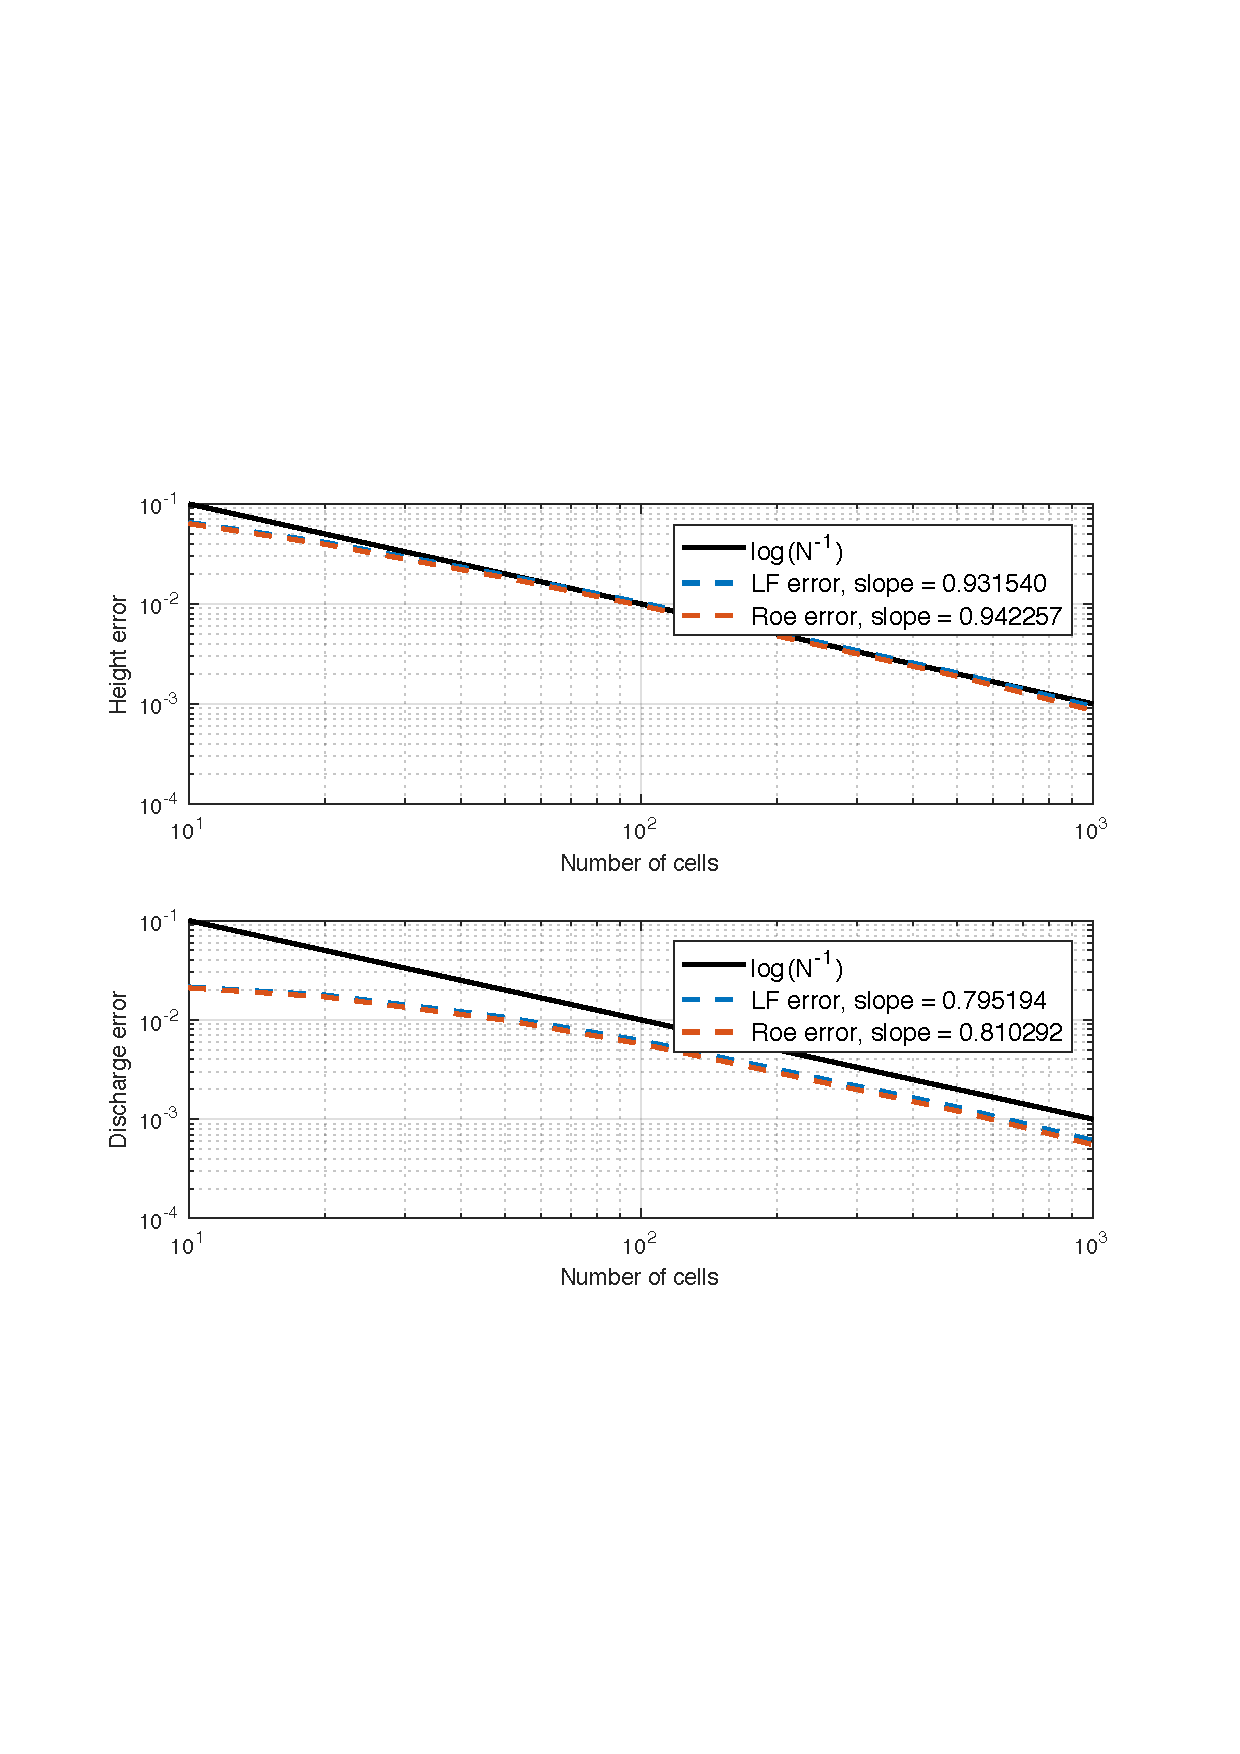
\includegraphics[width=11cm]{pictures/IC_2_error.pdf}
    \caption{LF and Roe methods errors, IC (5)}
    \label{fig:IC_2_errors}
\end{figure}

%IC 3
\begin{figure}[!htb]
    \centering
    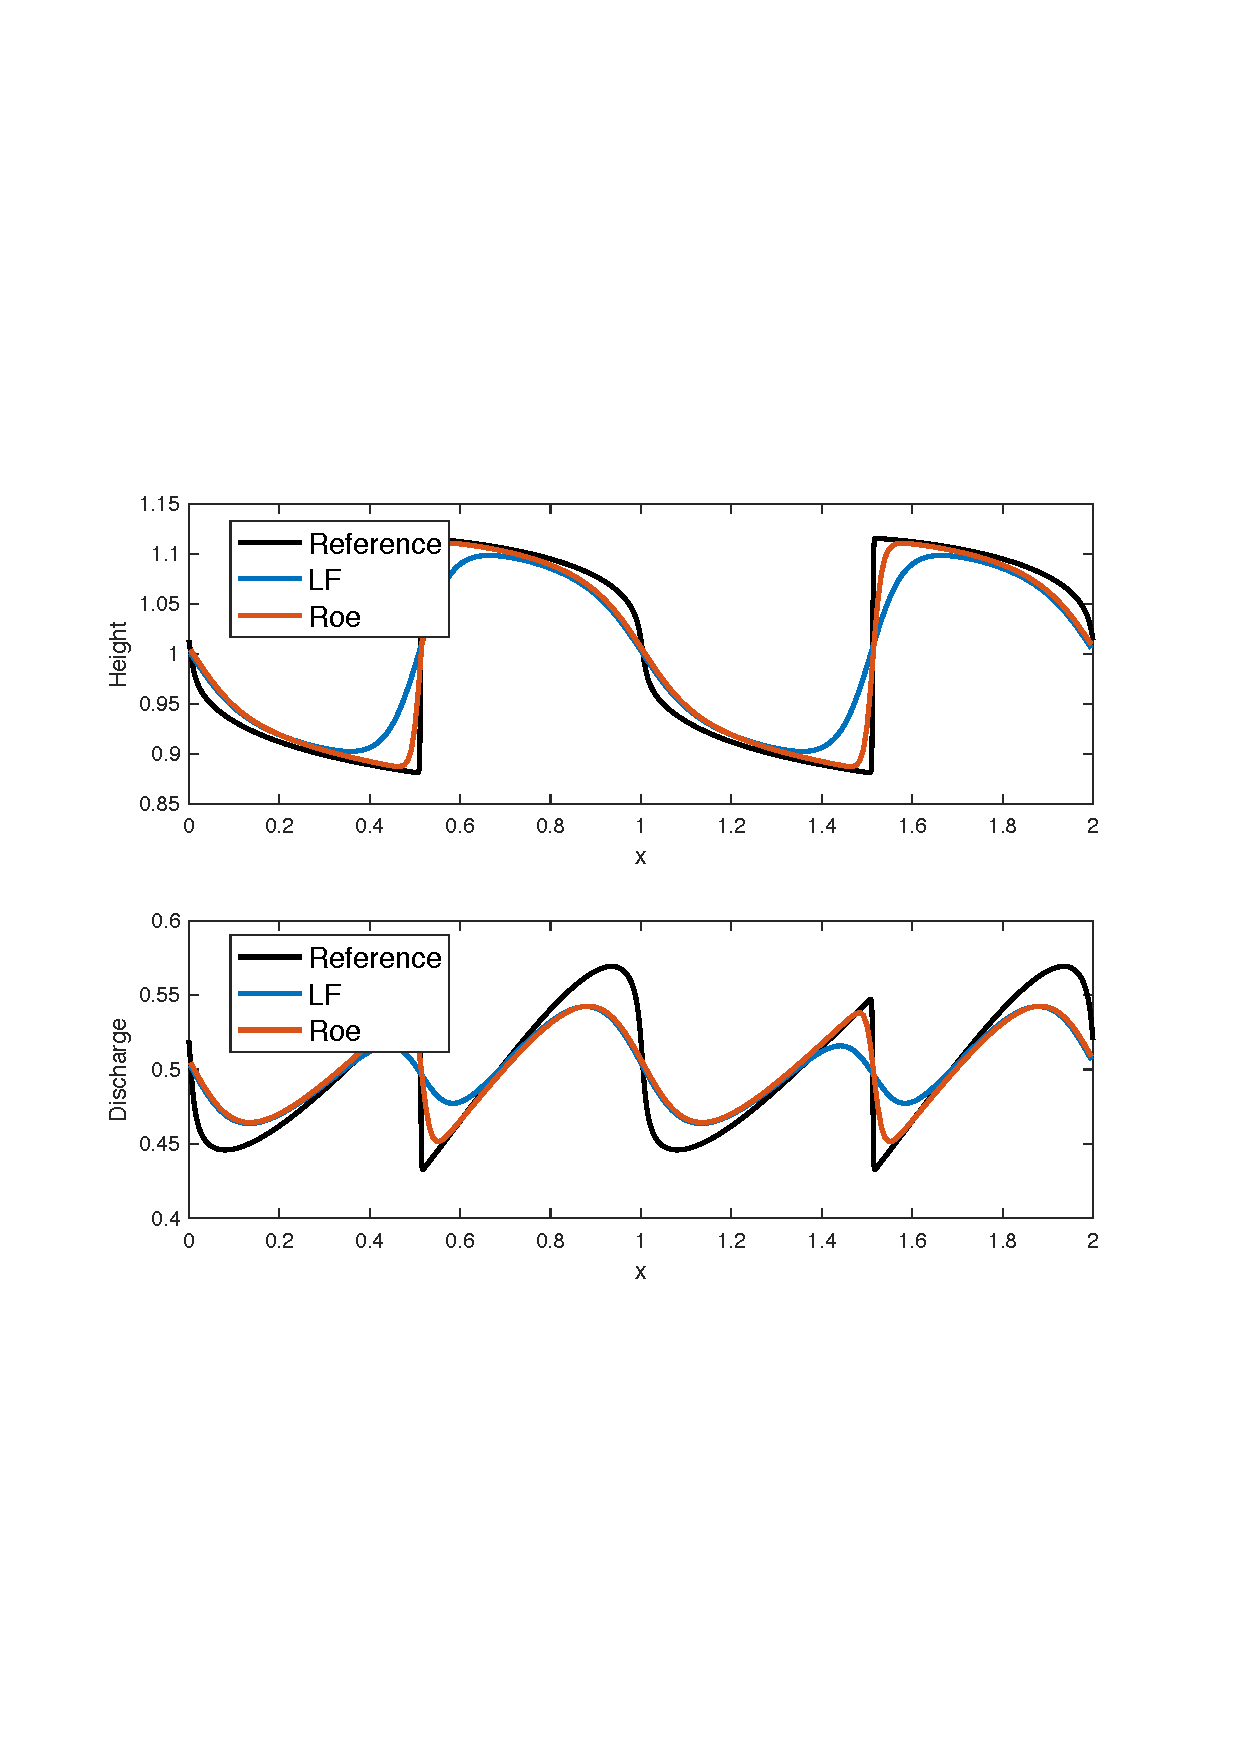
\includegraphics[width=11cm]{pictures/IC_3_250_cells.pdf}
    \caption{LF and Roe methods, 250 cells, IC (6)}
    \label{fig:IC_3_250_cells}
\end{figure}

\begin{figure}[!htb]
    \centering
    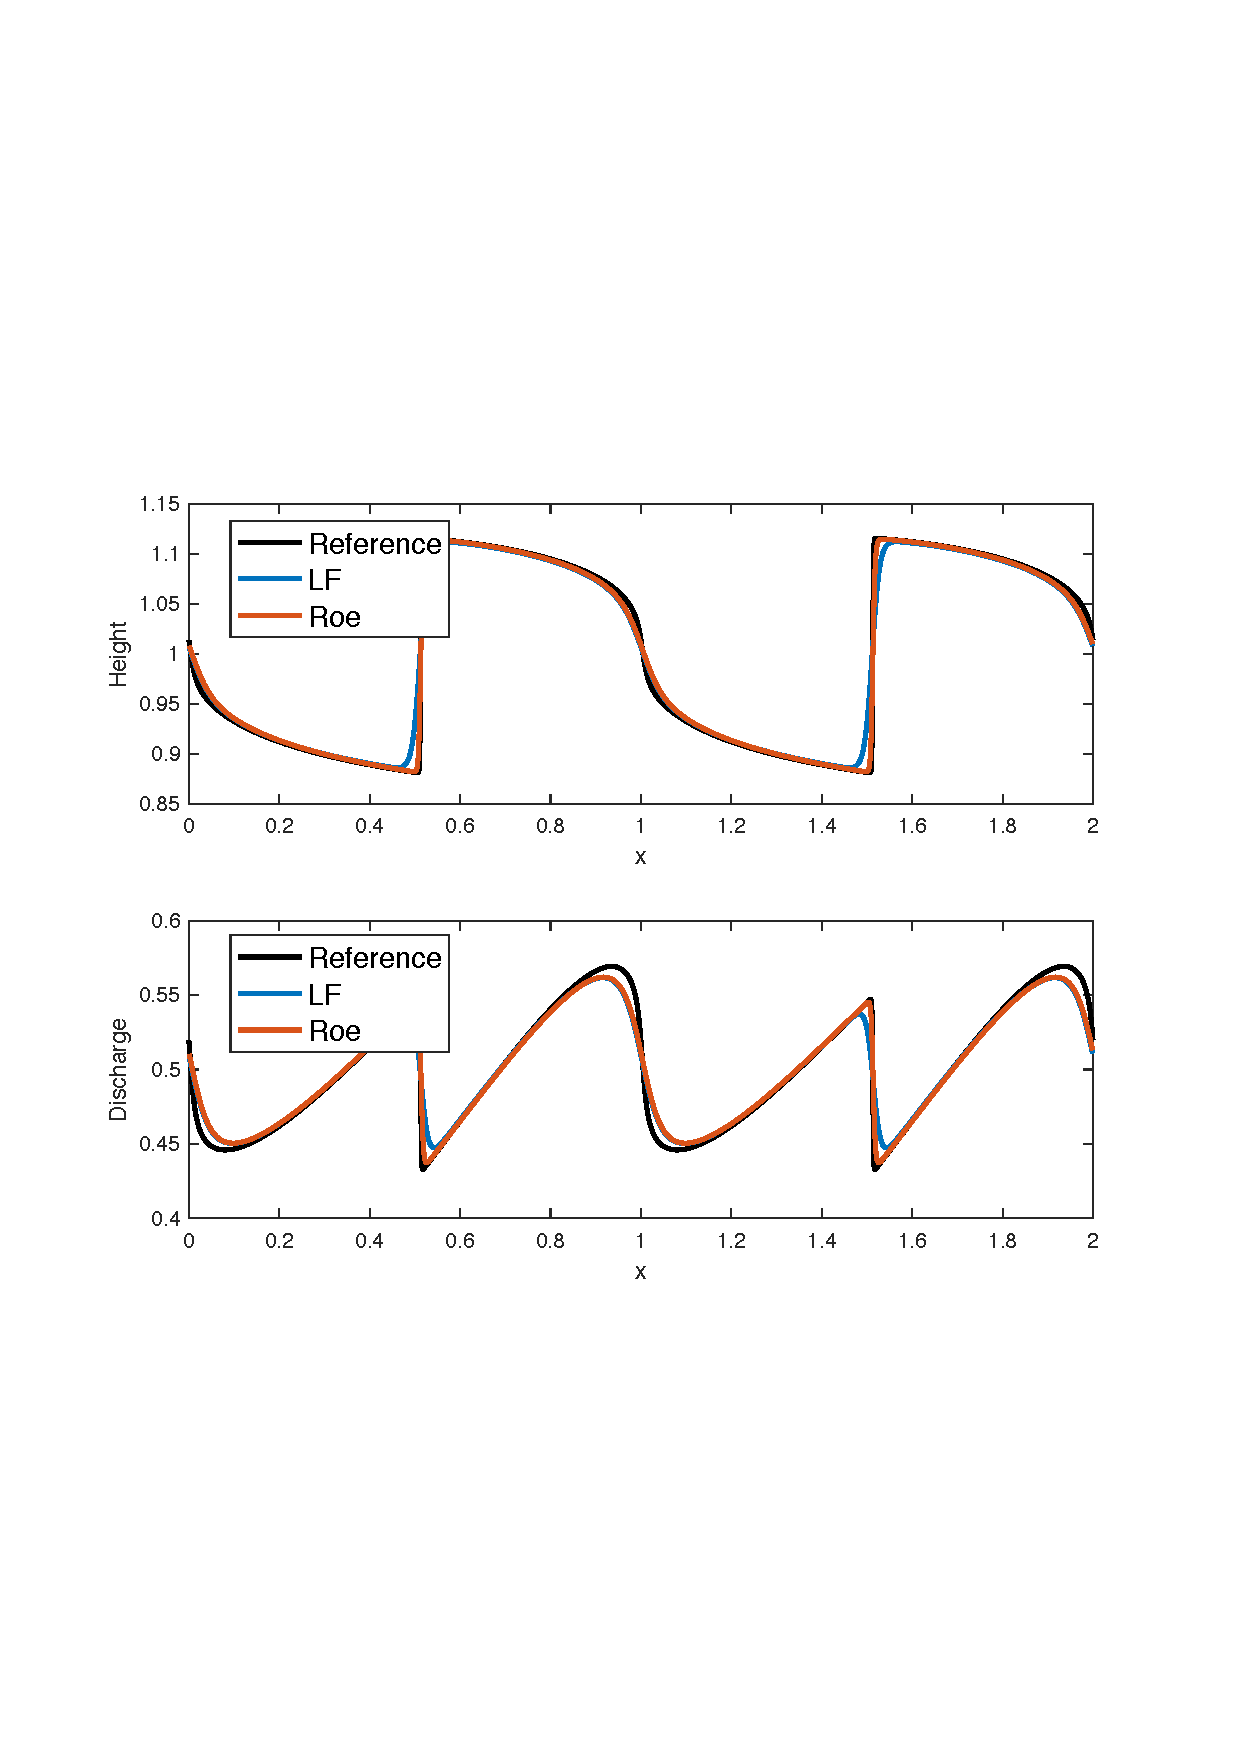
\includegraphics[width=11cm]{pictures/IC_3_1000_cells.pdf}
    \caption{LF and Roe methods, 1000 cells, IC (6)}
    \label{fig:IC_3_1000_cells}
\end{figure}

\begin{figure}[!htb]
    \centering
    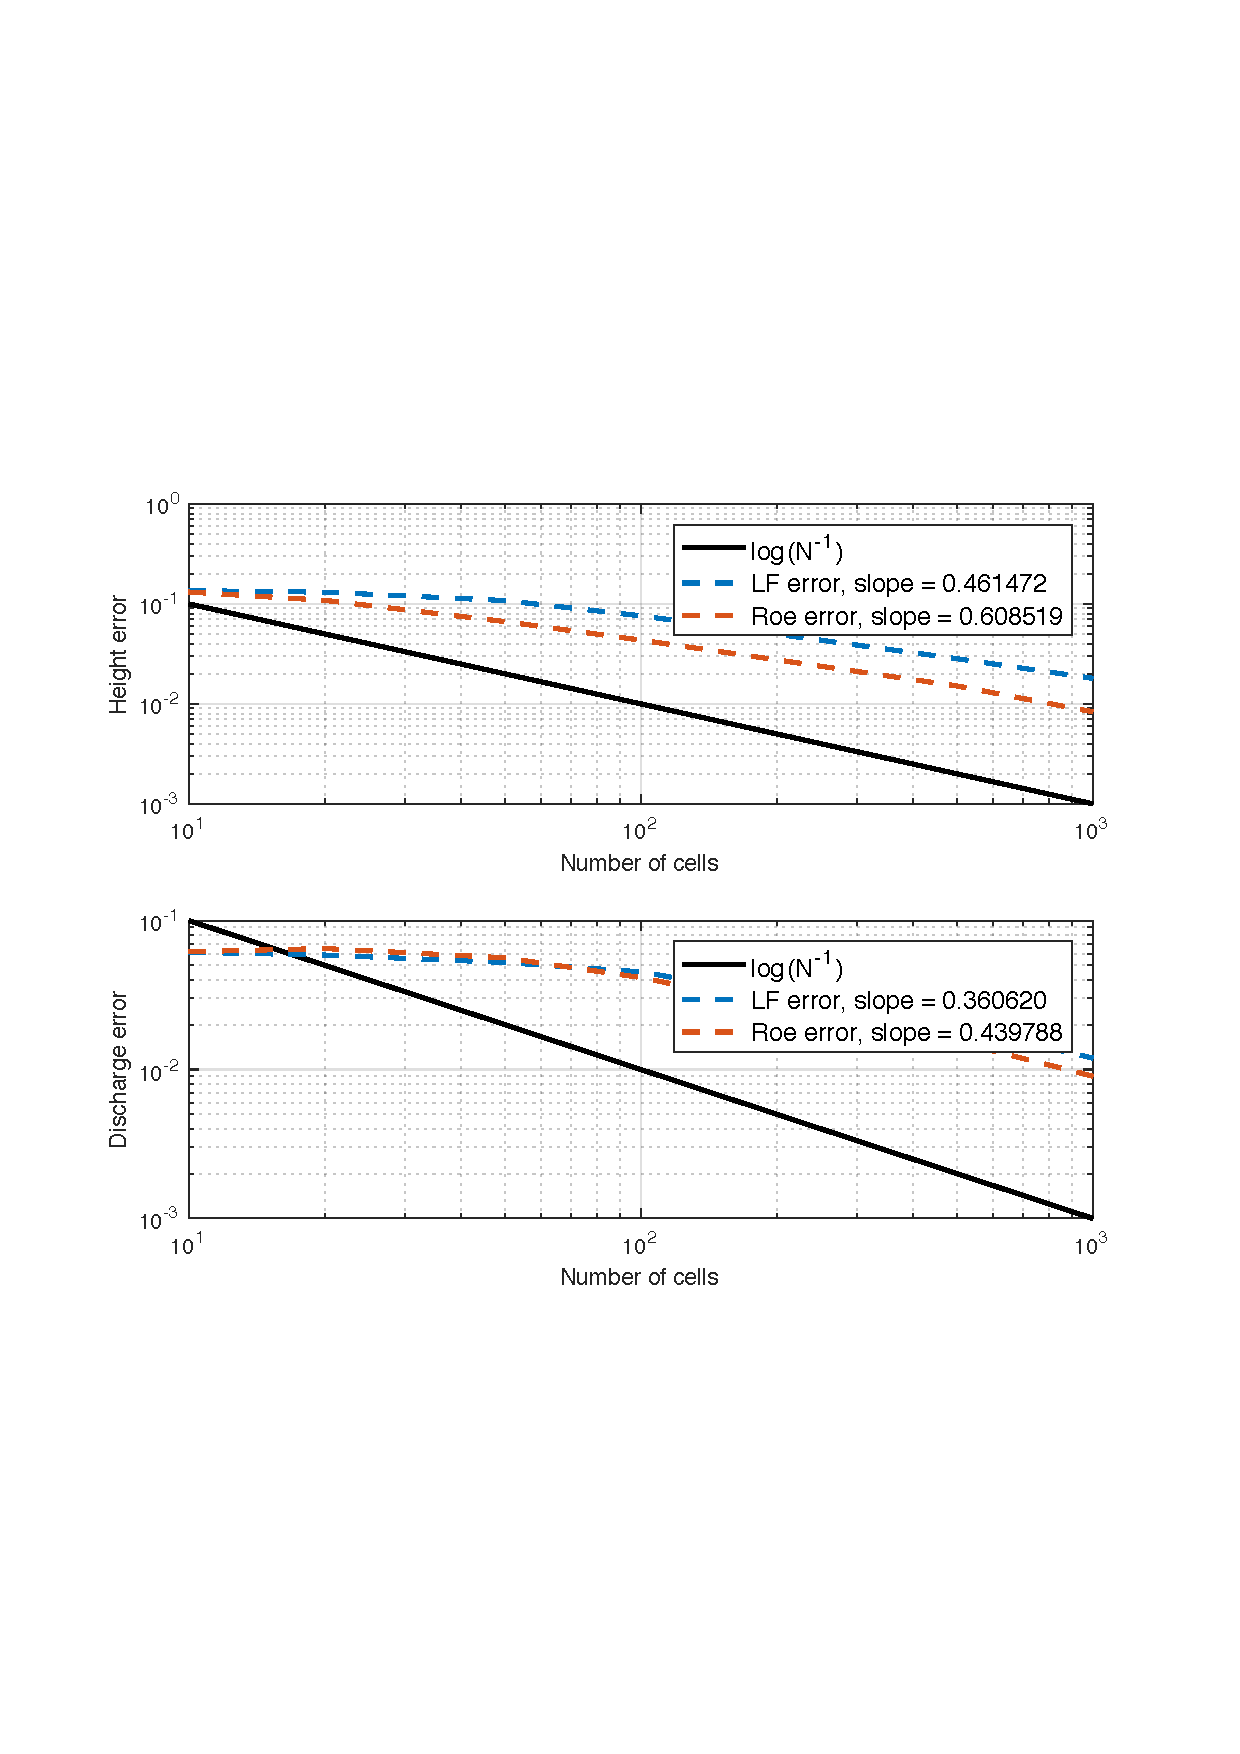
\includegraphics[width=11cm]{pictures/IC_3_error.pdf}
    \caption{LF and Roe methods errors, IC (6)}
    \label{fig:IC_3_errors}
\end{figure}

%IC 3
\begin{figure}[!htb]
    \centering
    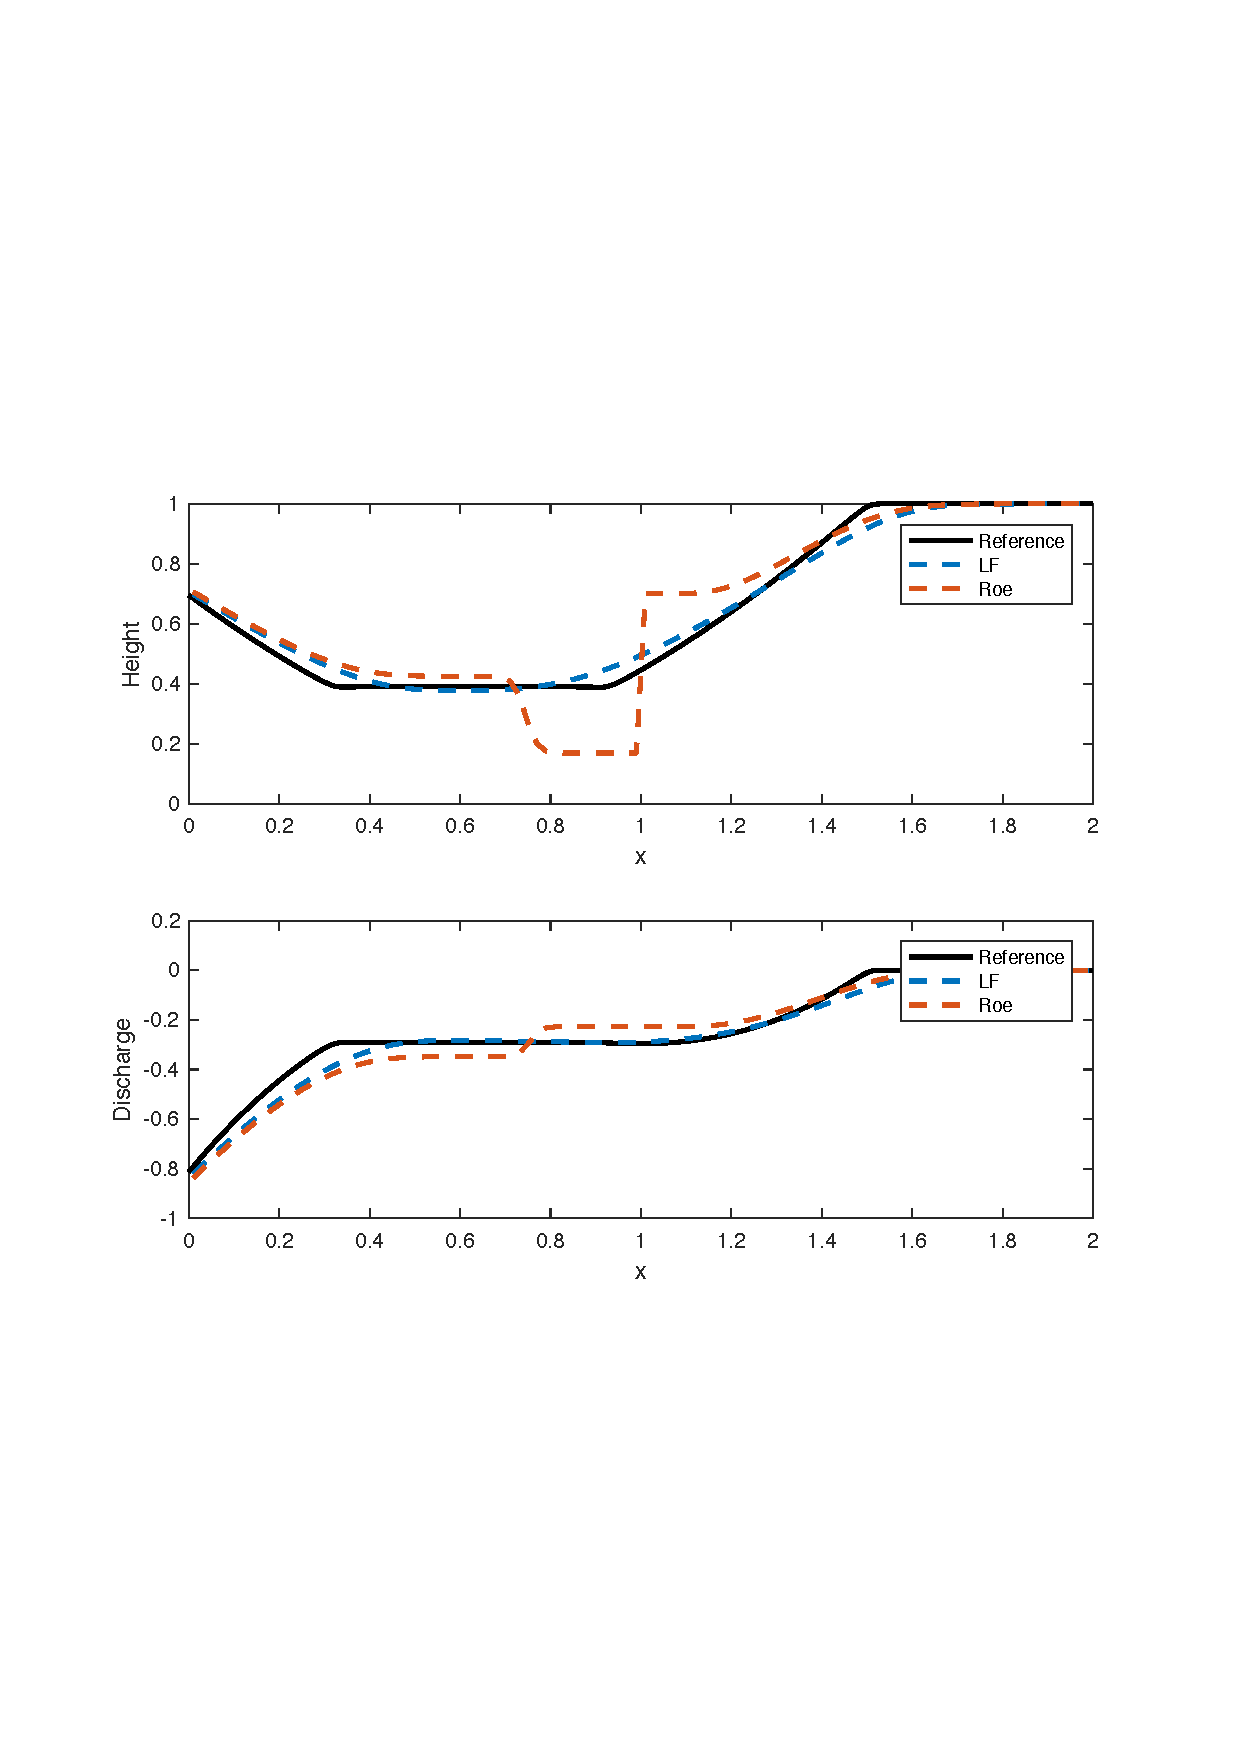
\includegraphics[width=11cm]{pictures/IC_4_100_cells.pdf}
    \caption{LF and Roe methods, 100 cells, IC (7)}
    \label{fig:IC_4_100_cells}
\end{figure}

\begin{figure}[!htb]
    \centering
    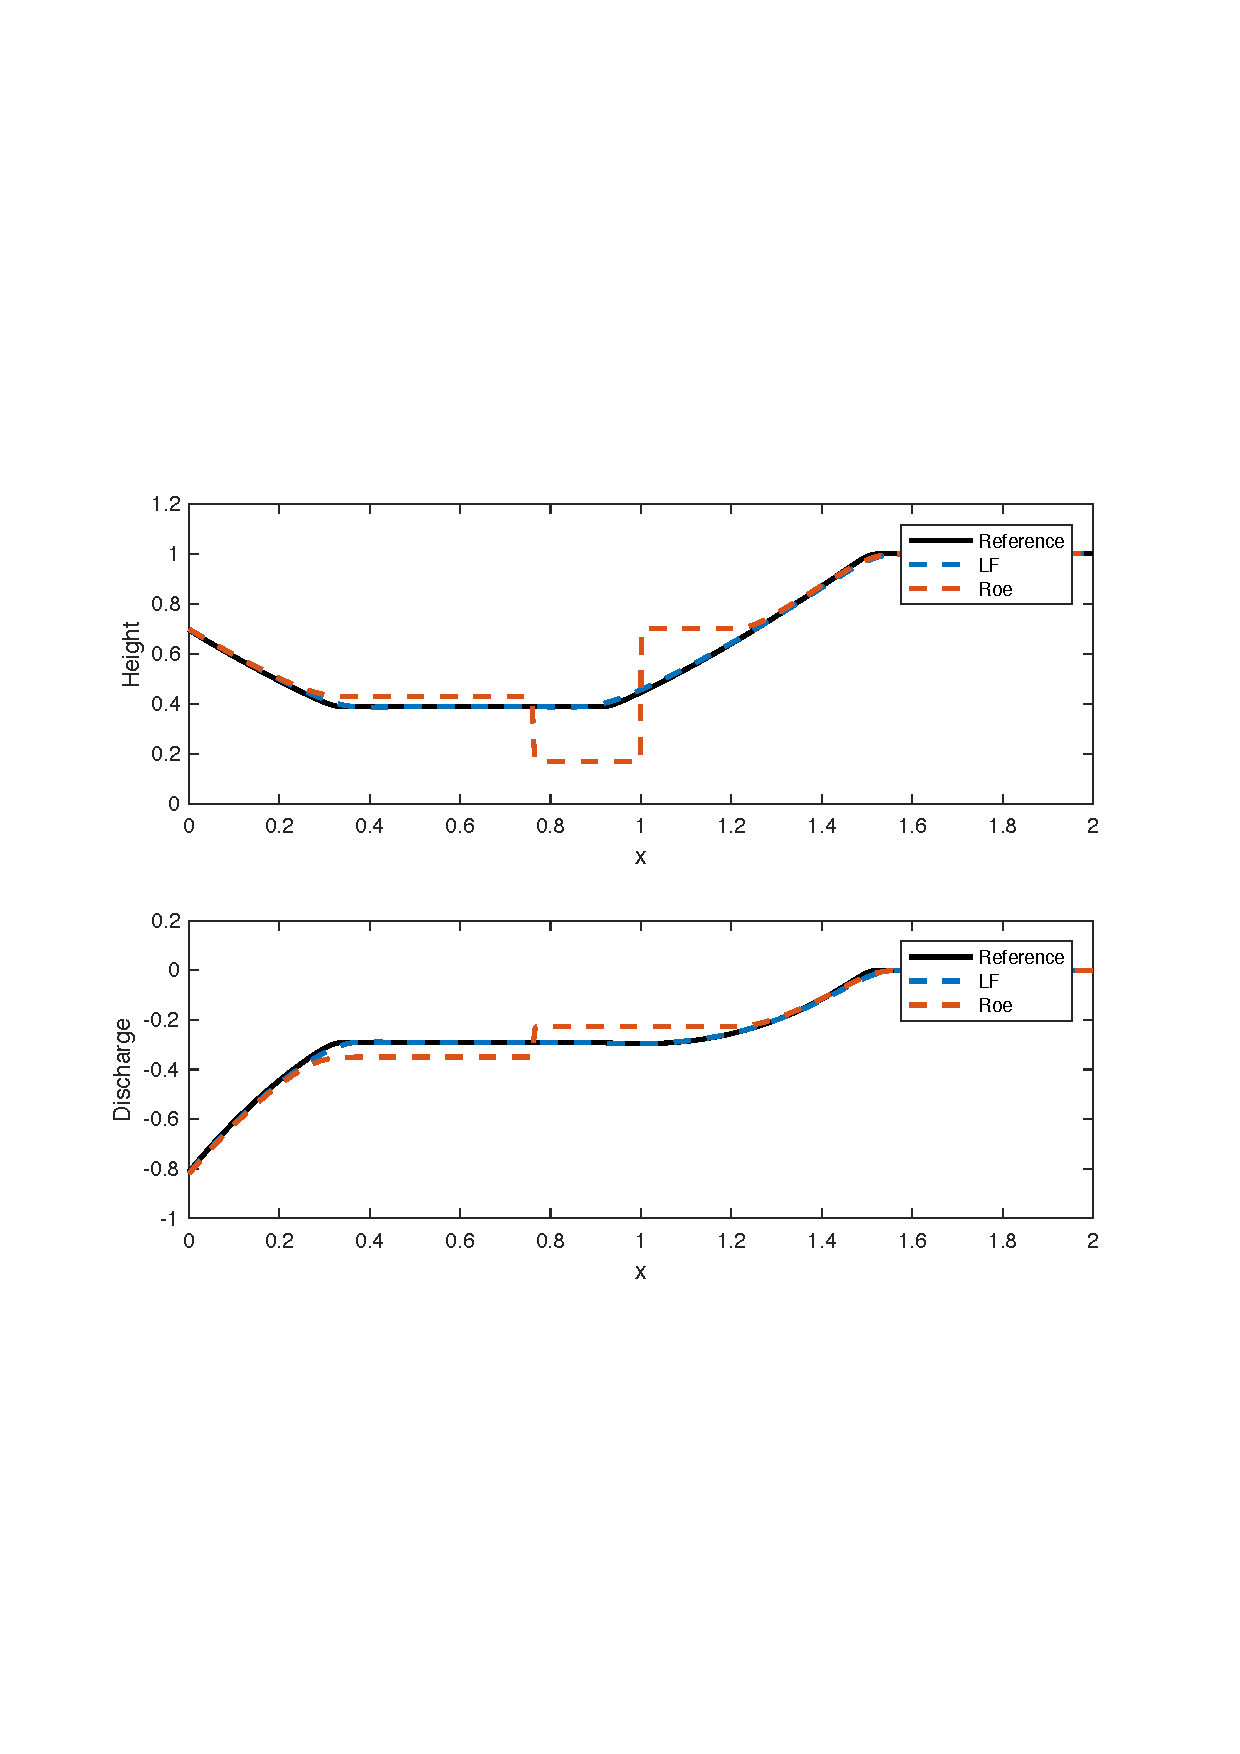
\includegraphics[width=11cm]{pictures/IC_4_1000_cells.pdf}
    \caption{LF and Roe methods, 1000 cells, IC (7)}
    \label{fig:IC_4_1000_cells}
\end{figure}

\begin{figure}[!htb]
    \centering
    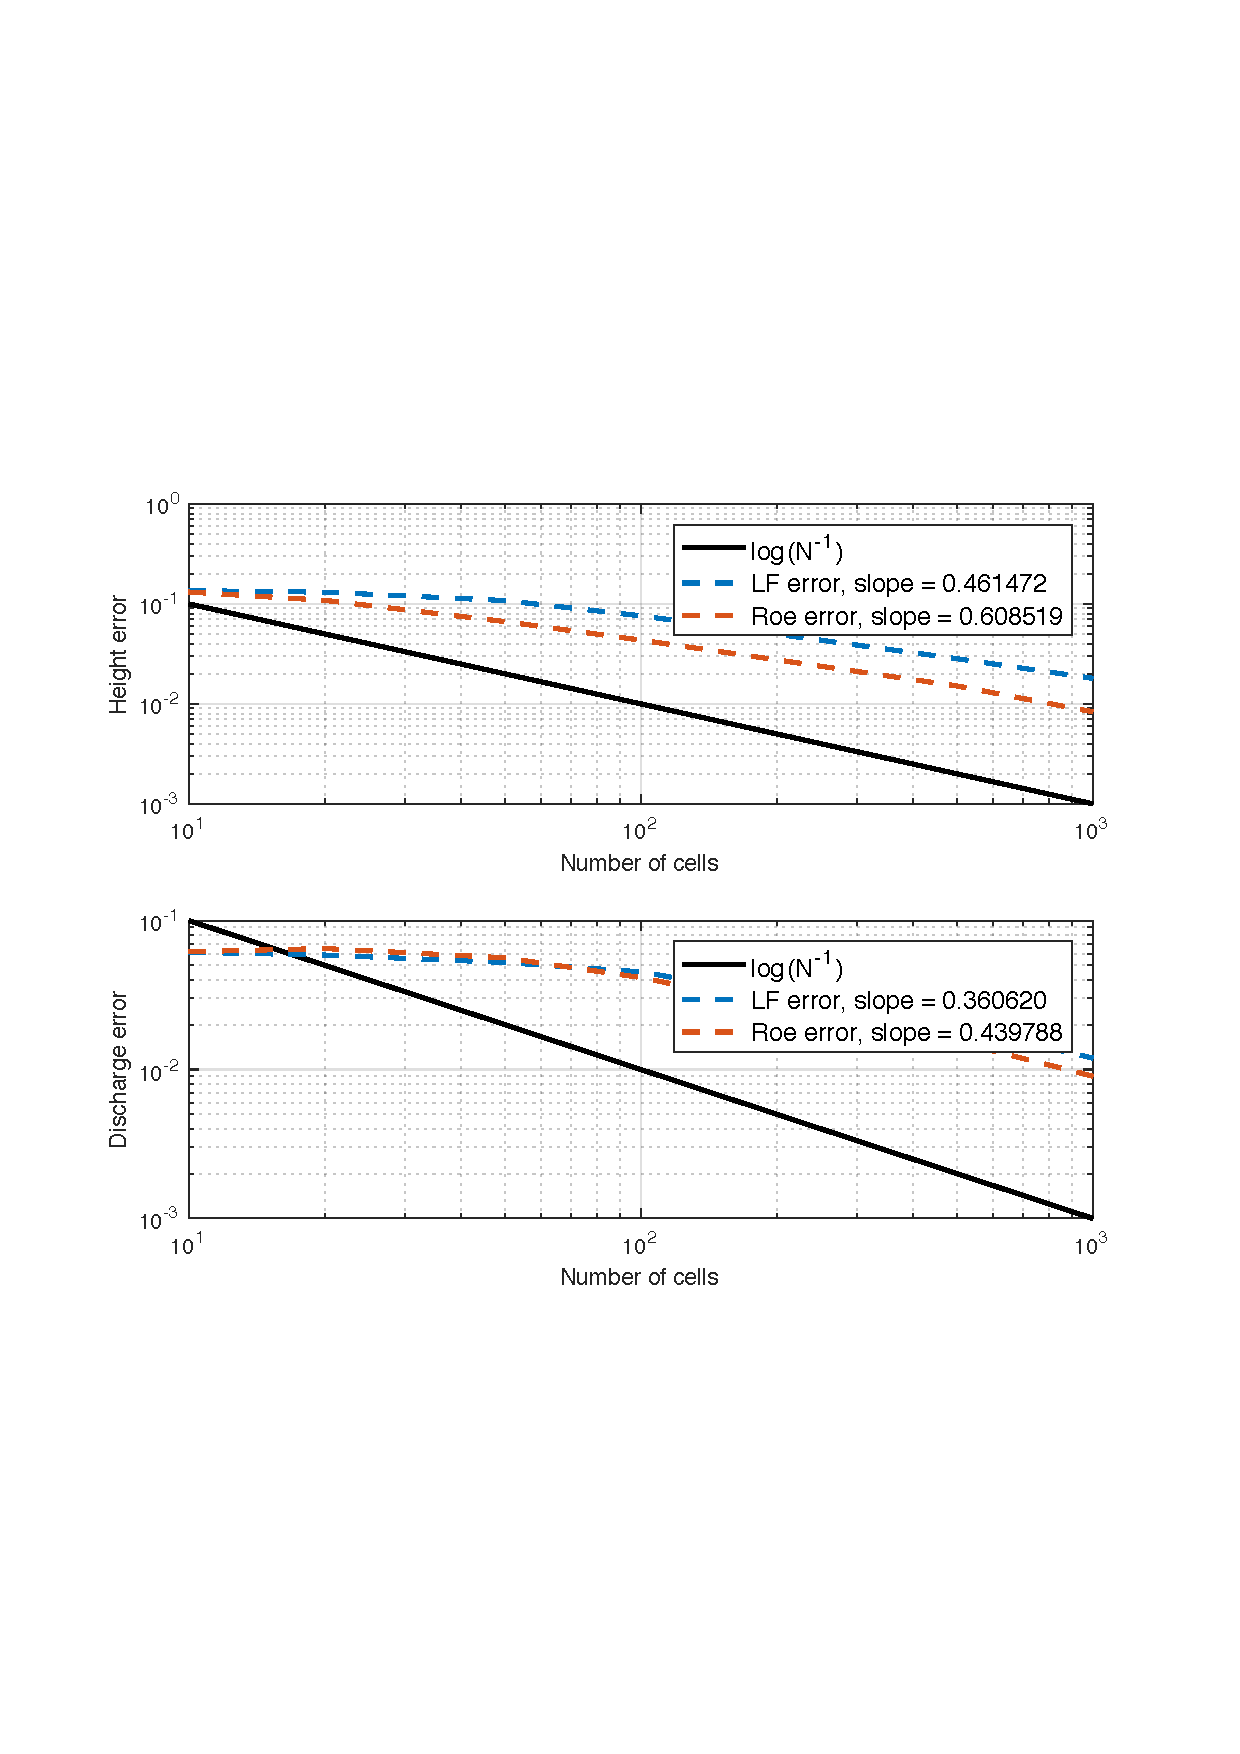
\includegraphics[width=11cm]{pictures/IC_3_error.pdf}
    \caption{LF and Roe methods errors, IC (7)}
    \label{fig:IC_4_errors}
\end{figure}




%------------------------------------------------------------------------

\afterpage{\blankpage}
\afterpage{\blankpage}
\afterpage{\blankpage}
\afterpage{\blankpage}
\afterpage{\blankpage}

\newpage
\appendix
%A.1 instead of A.a
\counterwithout*{subsection}{section}
\renewcommand{\thesubsection}{\thesection.\arabic{subsection}}
%Path to .m file
\lstset{inputpath=m}

\section{Utility functions}\label{utility}

\subsection{Applying boundary conditions}\label{BC}
\lstinputlisting{apply_bc.m}

\subsection{Initial conditions}\label{IC}
\lstinputlisting{Initial_conditions.m}

\subsection{Numerical flux}\label{flux}
\lstinputlisting{numerical_flux.m}

\subsection{Evaluating the RHS}\label{rhs}
\lstinputlisting{evalRHS.m}

\subsection{Godunov Flux}\label{G_flux}
\lstinputlisting{GodunovFlux.m}

\subsection{Solver}\label{solver}
\lstinputlisting{solver.m}

\subsection{Error}\label{error}
\lstinputlisting{p_error.m}

%------------------------------------------------------------------------
\section{Plotting solutions}\label{plot}


\subsection{Plot solution}\label{plot_sol}
\lstinputlisting{plots.m}

\subsection{Plot errors}\label{plot_err}
\lstinputlisting{errors.m}




\end{document}
